\chapter{Технологическая часть}

В технологическом разделе рассматриваются инструменты реализации и разработана архитектура программного обеспечения, декомпозиция программы, ключевые алгоритмы и пользовательский интерфейс.

\section{Выбор языка программирования и средств разработки}

Для реализации программного обеспечения был выбран язык программирования C++ и кроссплатформенный фреймворк Qt. Данный выбор обусловлен следующими соображениями:

\begin{enumerate}
	\item язык C++ был изучен при прохождении курса "Объектно-ориентированное программирование";
	
	\item объектно-ориентированный подход позволяет естественным образом представить сущности системы (частицы, системы частиц, камеру, источники света) в виде классов с инкапсуляцией данных и поведения;
	
	\item библиотека Qt предоставляет \cite{QtDocs}:
	\begin{itemize}
		\item средства для создания графического интерфейса (Qt Widgets);
		\item кроссплатформенность (Windows, Linux, macOS);
		\item встроенную поддержку 2D графики (QPainter, QImage);
		\item механизмы сигналов и слотов для обработки событий.
	\end{itemize}
\end{enumerate}

В качестве среды разработки использовался Qt Creator 8.0.1, система сборки -- CMake 3.25. Проект компилируется с использованием стандарта C++17.

\clearpage

\section{Организация модулей программы}

Программа состоит из следующих модулей:

\begin{enumerate}
	\item математические модули:
	\begin{itemize}
		\item \texttt{vector3.h/cpp} -- трёхмерные векторы и операции;
		\item \texttt{matrix4x4.h/cpp} -- матрицы 4×4 и преобразования.
	\end{itemize}
	
	\item модули моделирования:
	\begin{itemize}
		\item \texttt{particle.h/cpp} -- класс отдельной частицы;
		\item \texttt{particlesystem.h/cpp} -- система частиц;
		\item \texttt{scene.h/cpp} -- управление сценой;
		\item \texttt{camera.h/cpp} -- виртуальная камера;
		\item \texttt{light.h/cpp} -- источник освещения.
	\end{itemize}
	
	\item модули визуализации:
	\begin{itemize}
		\item \texttt{firecanvas.h/cpp} -- виджет рендеринга с реализацией z-буфера.
	\end{itemize}
	
	\item модули интерфейса:
	\begin{itemize}
		\item \texttt{mainwindow.h/cpp} -- главное окно приложения;
		\item \texttt{main.cpp} -- точка входа.
	\end{itemize}
\end{enumerate}

На рисунке \ref{fig:compoment-diagram} представлена диаграмма компонентов программы.

\begin{figure}[h!]
	\centering
	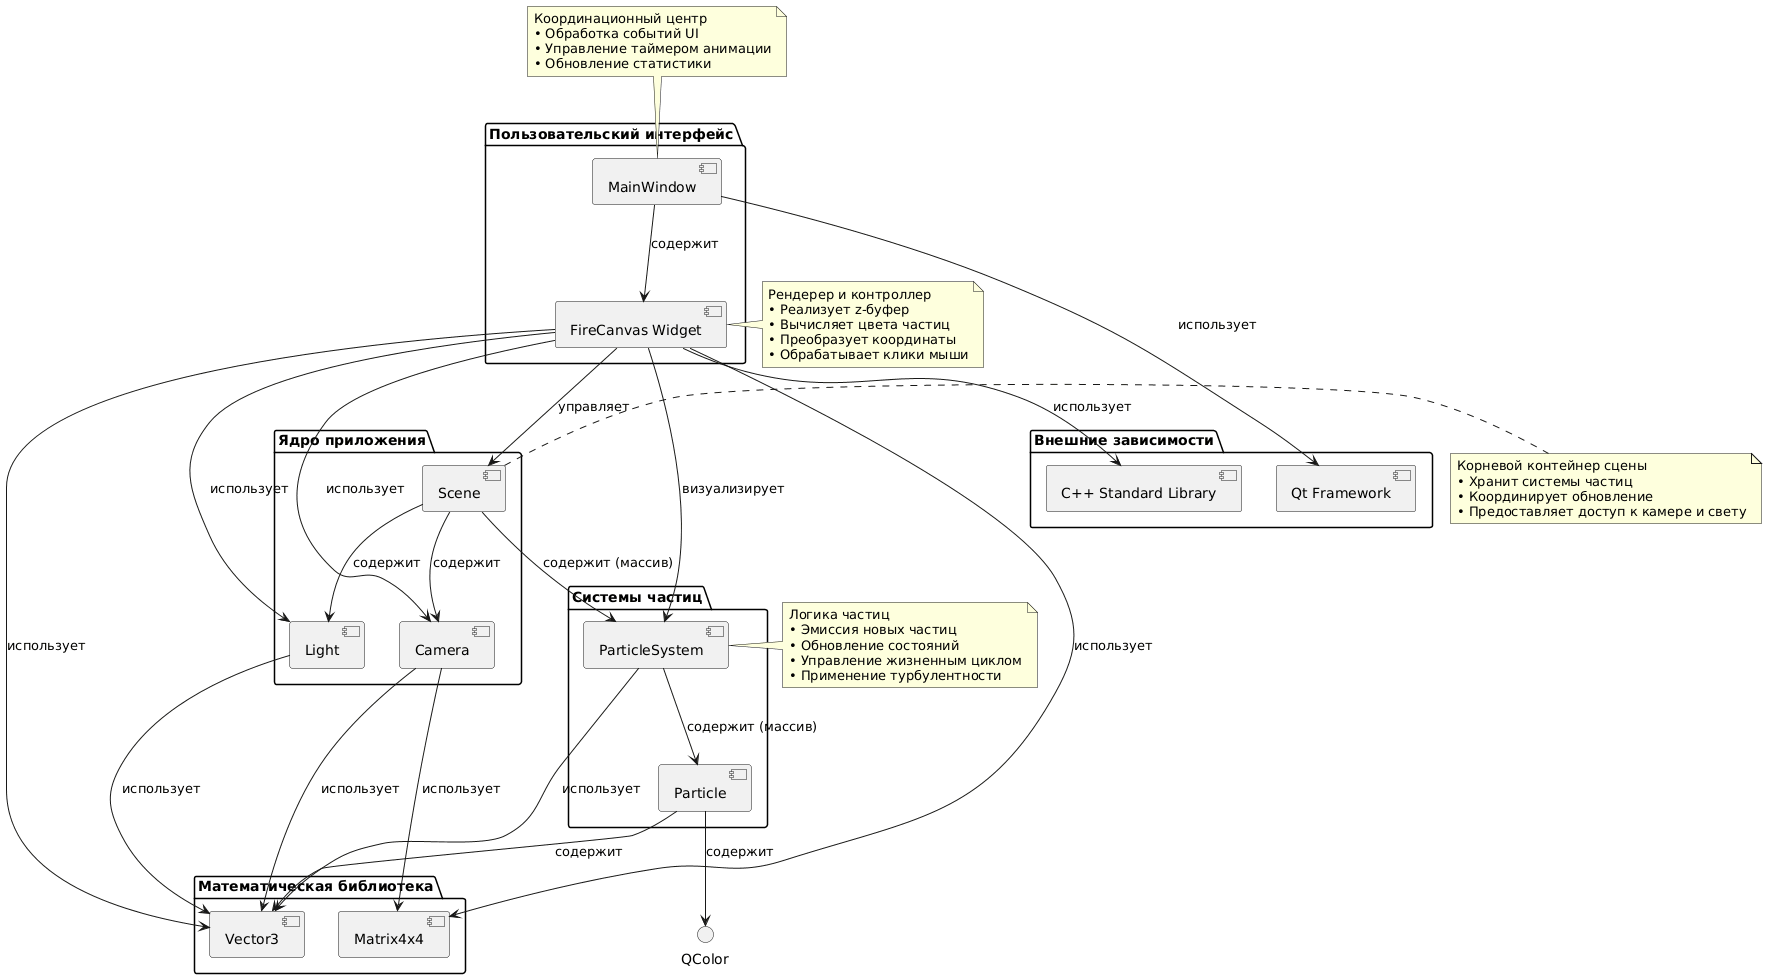
\includegraphics[width=0.95\textwidth]{comp.png}
	\caption{Диаграмма компонентов системы визуализации огня}
	\label{fig:compoment-diagram}
\end{figure}

\clearpage

\section{Структура классов программного обеспечения}

На рисунке \ref{fig:class-diagram} представлена диаграмма классов основных сущностей системы.

\begin{figure}[h!]
	\centering
	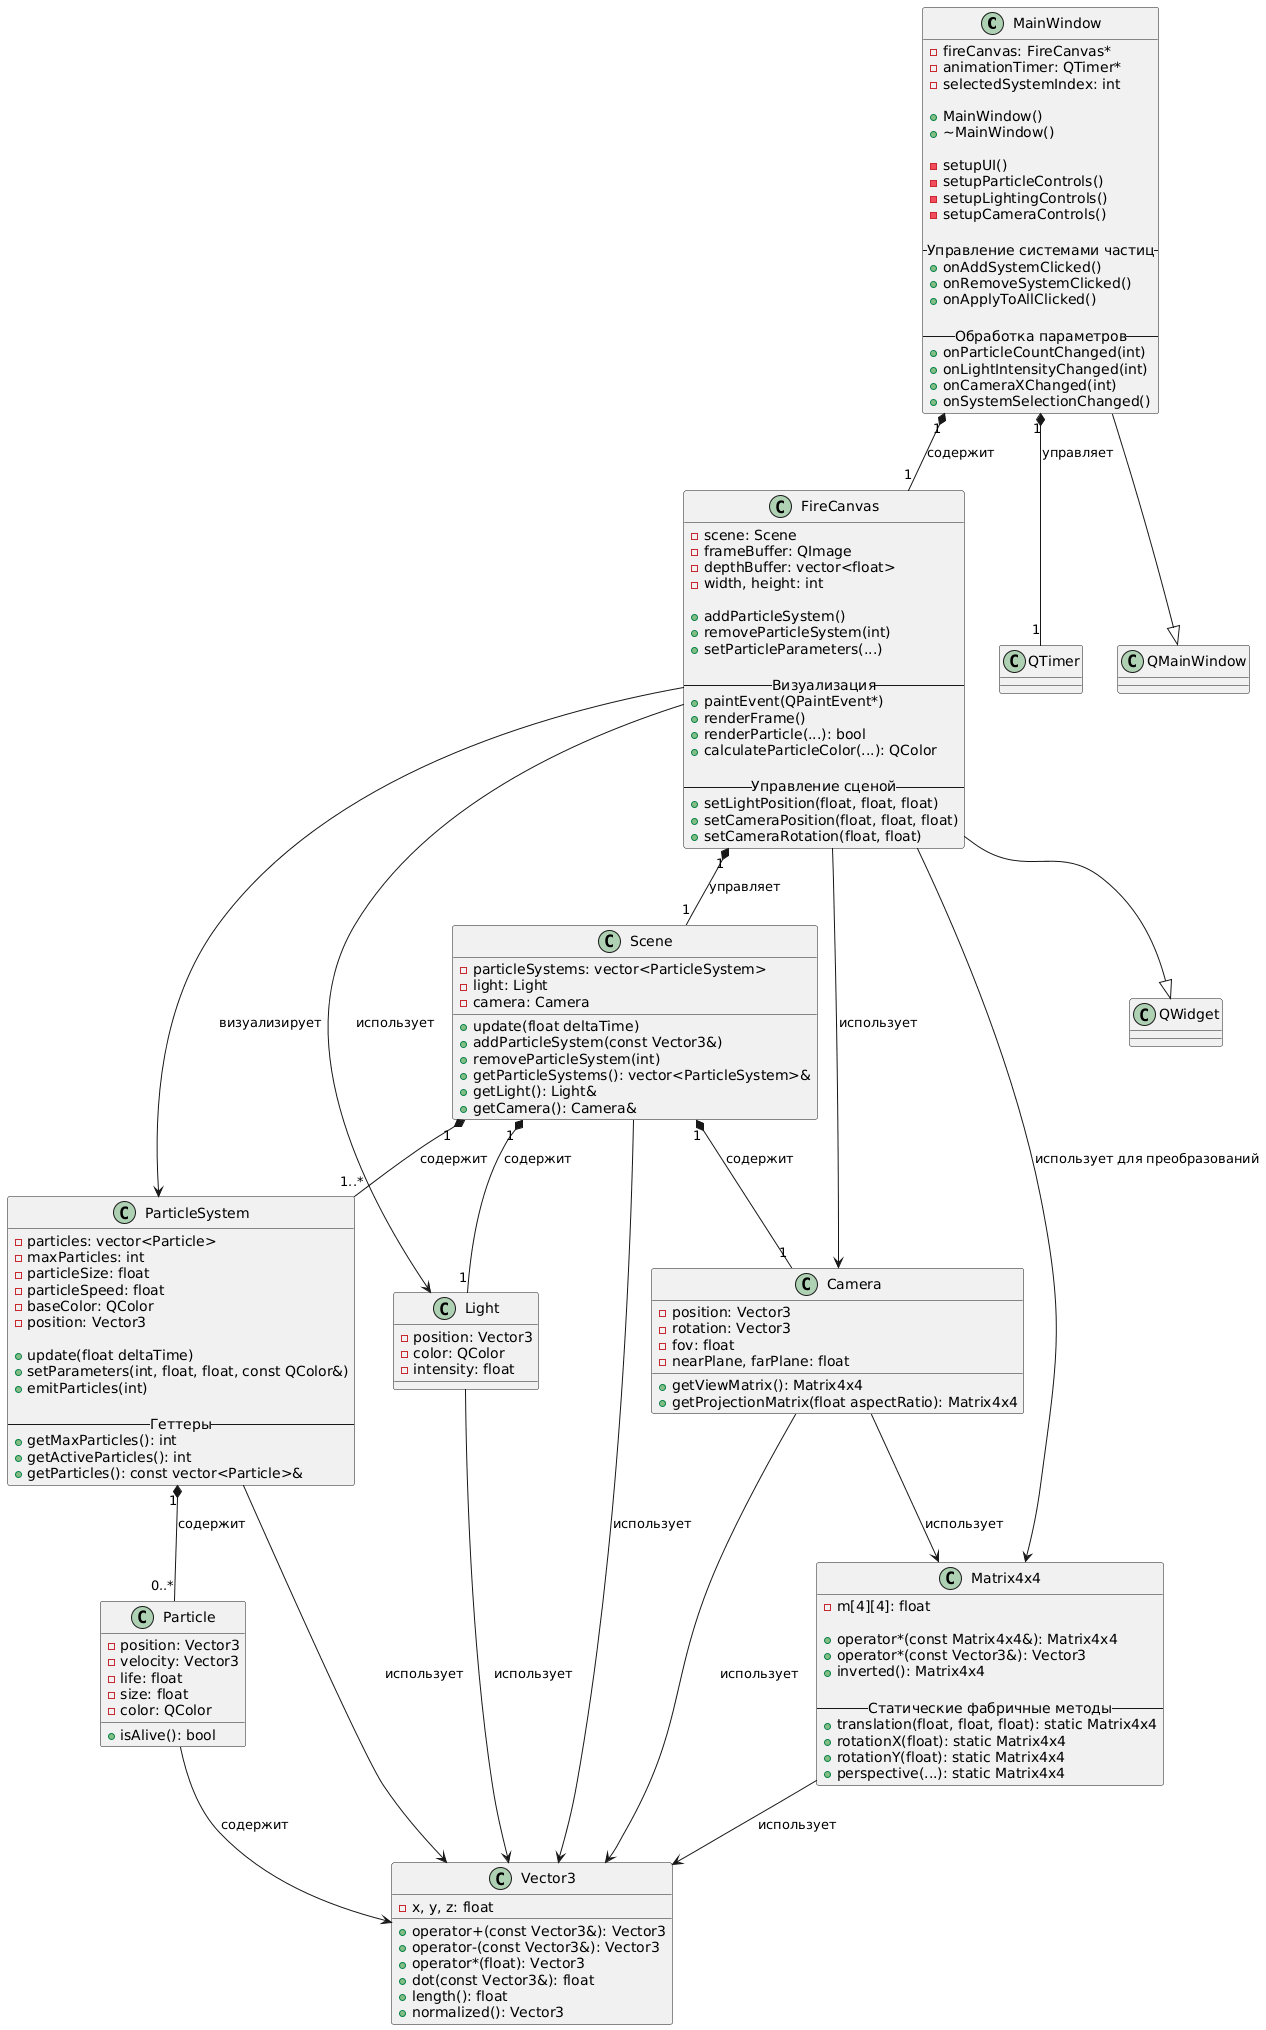
\includegraphics[width=0.8\textwidth]{uml.png}
	\caption{Диаграмма классов системы визуализации огня}
	\label{fig:class-diagram}
\end{figure}

\clearpage

\section{Реализация ключевых алгоритмов}

\subsection{Алгоритм обновления системы частиц}

Метод \texttt{update} класса \texttt{ParticleSystem} реализует обновление состояния системы частиц за временной шаг. В листинге \ref{lst:3.1} представлена реализация данного метода.

\begin{lstlisting}[language=C++, caption={Реализация метода обновления системы частиц}, label={lst:3.1},captionpos=b]
	void ParticleSystem::update(float deltaTime) {
		timeSinceLastEmission += deltaTime;
		int particlesToEmit = static_cast<int>(emissionRate * deltaTime);
		if (particlesToEmit > 0 && 
		particles.size() < static_cast<size_t>(maxParticles)) {
			emitParticles(particlesToEmit);
		}
		
		for (auto &particle : particles) {
			if (!particle.isAlive()) continue;
			
			particle.position = particle.position + 
			particle.velocity * deltaTime * particleSpeed;
			
			const float decayRate = 0.4f;
			particle.life -= decayRate * deltaTime;
			
			if (!particle.isAlive()) continue;
			
			particle.velocity.x += (std::rand() % 100 - 50) / 500.0f * deltaTime;
			particle.velocity.z += (std::rand() % 100 - 50) / 500.0f * deltaTime;
			
			updateParticleVisuals(particle);
		}
		
		if (std::rand() % 1000 == 0) {
			particles.erase(std::remove_if(particles.begin(), particles.end(),
			[](const Particle &p) { return !p.isAlive(); }), 
			particles.end());
		}
	}
\end{lstlisting}

\clearpage

\subsection{Алгоритм вычисления цвета частицы с учётом освещения}

Метод \texttt{calculateParticleColor} класса \texttt{FireCanvas} реализует вычисление конечного цвета частицы на основе принятой модели освещения. В листинге \ref{lst:3.2} представлена реализация данного метода.

\begin{lstlisting}[language=C++, caption={Вычисление цвета частицы с учётом освещения}, label={lst:3.2},captionpos=b]
	QColor FireCanvas::calculateParticleColor(const Particle &particle) {
		Light &light = scene.getLight();
		
		QColor baseColor = particle.color;
		float life = std::max(0.0f, std::min(1.0f, particle.life));
		baseColor.setAlphaF(life);
		
		Vector3 toLight = light.position - particle.position;
		float distanceToLight = toLight.length();
		
		float attenuation = 1.0f / (1.0f + 0.01f * 
		distanceToLight * distanceToLight);
		
		float emissionFactor = 1.0f;
		float externalFactor = light.intensity * attenuation;
		float totalFactor = emissionFactor + externalFactor;
		
		float r = baseColor.redF() * totalFactor;
		float g = baseColor.greenF() * totalFactor;
		float b = baseColor.blueF() * totalFactor;
		float a = baseColor.alphaF();
		
		r = std::min(1.0f, r);
		g = std::min(1.0f, g);
		b = std::min(1.0f, b);
		
		QColor result;
		result.setRgbF(r, g, b, a);
		return result;
	}
\end{lstlisting}

\clearpage

\subsection{Алгоритм z-буфера с аддитивным смешиванием}

Метод \texttt{renderParticle} класса \texttt{FireCanvas} реализует рендеринг отдельной частицы с использованием алгоритма z-буфера. В листинге \ref{lst:3.3} представлена реализация данного метода.

\begin{lstlisting}[language=C++, caption={Рендеринг частицы с использованием z-буфера}, label={lst:3.3},captionpos=b]
	bool FireCanvas::renderParticle(const Particle &particle,
	const Matrix4x4 &viewProjection) {
		Vector3 screenPos = viewProjection * particle.position;
		
		if (screenPos.z < 0 || screenPos.z > 1 || 
		screenPos.x < -1 || screenPos.x > 1 ||
		screenPos.y < -1 || screenPos.y > 1) {
			return false;
		}
		
		int x = (screenPos.x + 1) * width / 2;
		int y = (1 - screenPos.y) * height / 2;
		
		int index = y * width + x;
		if (screenPos.z < depthBuffer[index]) {
			depthBuffer[index] = screenPos.z;
			
			drawBillboard(x, y, screenPos.z, 
			static_cast<int>(particle.size * 100), 
			calculateParticleColor(particle));
			return true;
		}
		return false;
	}
\end{lstlisting}

\clearpage

\section{Интерфейс пользователя}

Интерфейс программы разделён на логические блоки управления, организованные во вкладках. На рисунках \ref{fig:ui-main}--\ref{fig:ui-stats} представлены основные элементы интерфейса.

Область визуализации (левый блок) отображает 3D-сцену с системами частиц в реальном времени. Панель управления (правый блок) содержит четыре вкладки: «Частицы», «Свет», «Камера» и «Статистика».

Пользователь может добавлять новые системы частиц по клику в области визуализации. Все изменения параметров отражаются на визуализации, обеспечивая работу в реальном времени. Интерфейс использует тёмную цветовую схему для снижения нагрузки на глаза при длительной работе.

\begin{figure}[h!]
	\centering
	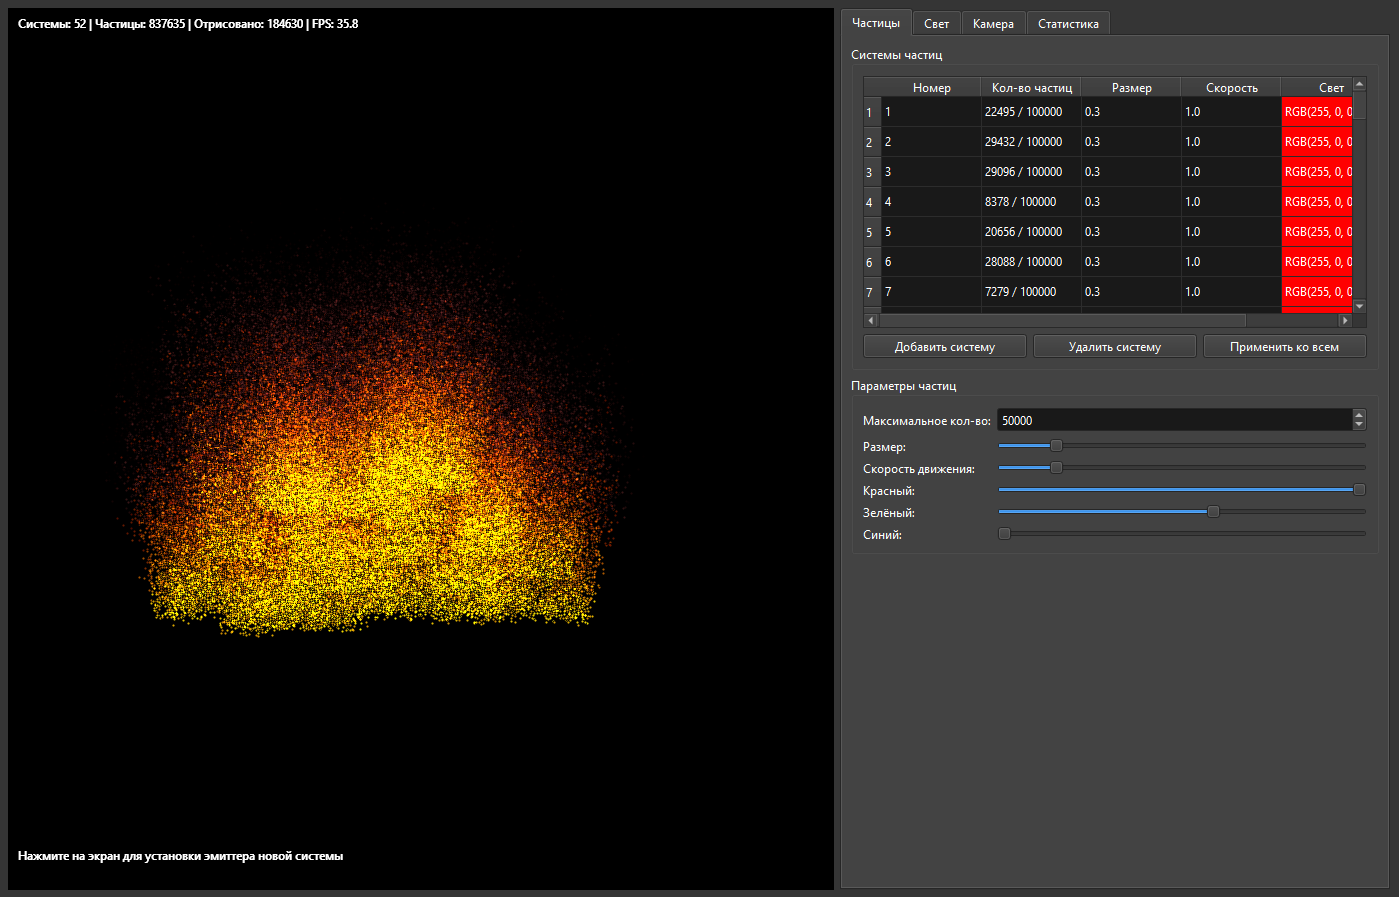
\includegraphics[width=0.99\textwidth]{ui_main.png}
	\caption{Главное окно программы с областью визуализации и панелью управления}
	\label{fig:ui-main}
\end{figure}

\clearpage

Вкладка "Частицы" содержит таблицу систем частиц с текущими параметрами, элементы управления параметрами выбранной системы, кнопки добавления и удаления систем, а также ползунки для настройки цвета (RGB). Интерфейс позволяет управлять несколькими независимыми системами частиц, каждая из которых представляет отдельный источник пламени.

\begin{figure}[h!]
	\centering
	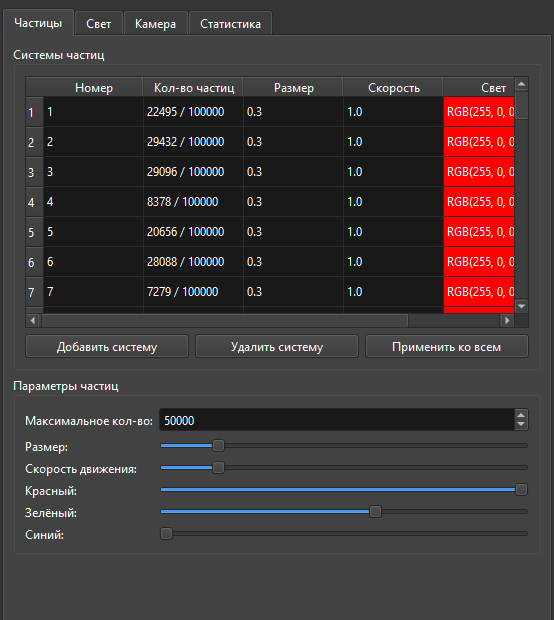
\includegraphics[width=0.5\textwidth]{ui_particles.png}
	\caption{Вкладка управления частицами с таблицей систем и элементами настройки}
	\label{fig:ui-particles}
\end{figure}

Вкладка "Свет" предоставляет элементы для настройки позиции источника света (координаты X, Y, Z), регулятор интенсивности освещения и отображение текущих координат. Пользователь может интерактивно изменять параметры внешнего освещения и наблюдать их влияние на визуализацию пламени.

\begin{figure}[h!]
	\centering
	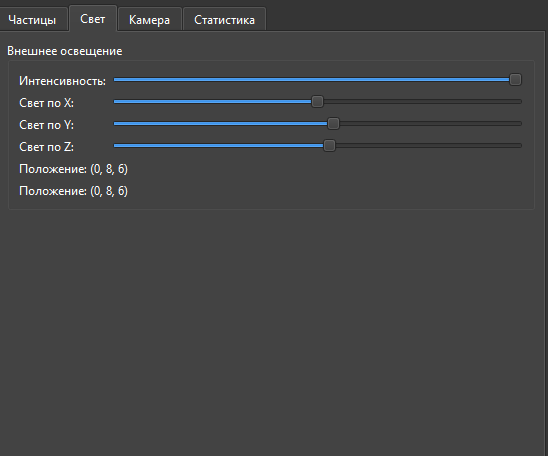
\includegraphics[width=0.55\textwidth]{ui_light.png}
	\caption{Вкладка управления освещением с настройками источника света}
	\label{fig:ui-light}
\end{figure}


Вкладка "Камера" содержит элементы управления позицией камеры, регулировки углов поворота и настройки поля зрения (FOV). Это позволяет пользователю свободно перемещаться по сцене и выбирать оптимальный ракурс для наблюдения

\begin{figure}[h!]
	\centering
	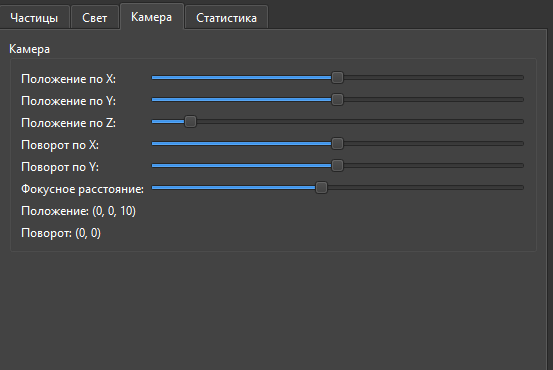
\includegraphics[width=0.5\textwidth]{ui_camera.png}
	\caption{Вкладка управления камерой с настройками позиции и ориентации}
	\label{fig:ui-camera}
\end{figure}

Вкладка "Статистика" отображает текущий FPS, общее количество частиц и количество активных систем. Эта информация позволяет отслеживать производительность программы при различных настройках и количестве частиц.

\begin{figure}[h!]
	\centering
	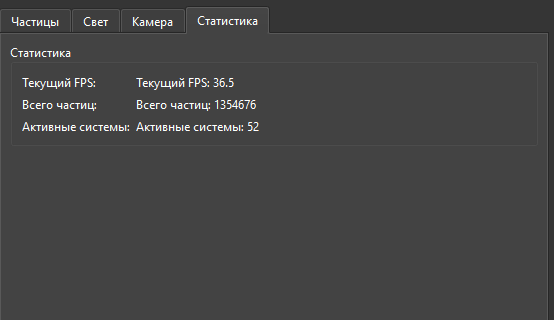
\includegraphics[width=0.5\textwidth]{ui_stats.png}
	\caption{Вкладка статистики с информацией о производительности системы}
	\label{fig:ui-stats}
\end{figure}

\clearpage

\section{Результаты работы программного обеспечения}

Программное обеспечение позволяет визуализировать трёхмерный огонь с различными параметрами систем частиц, освещения и камеры. На рисунках \ref{fig:research-1}--\ref{fig:research-6} представлены примеры работы программы.

\begin{figure}[h!]
	\centering
	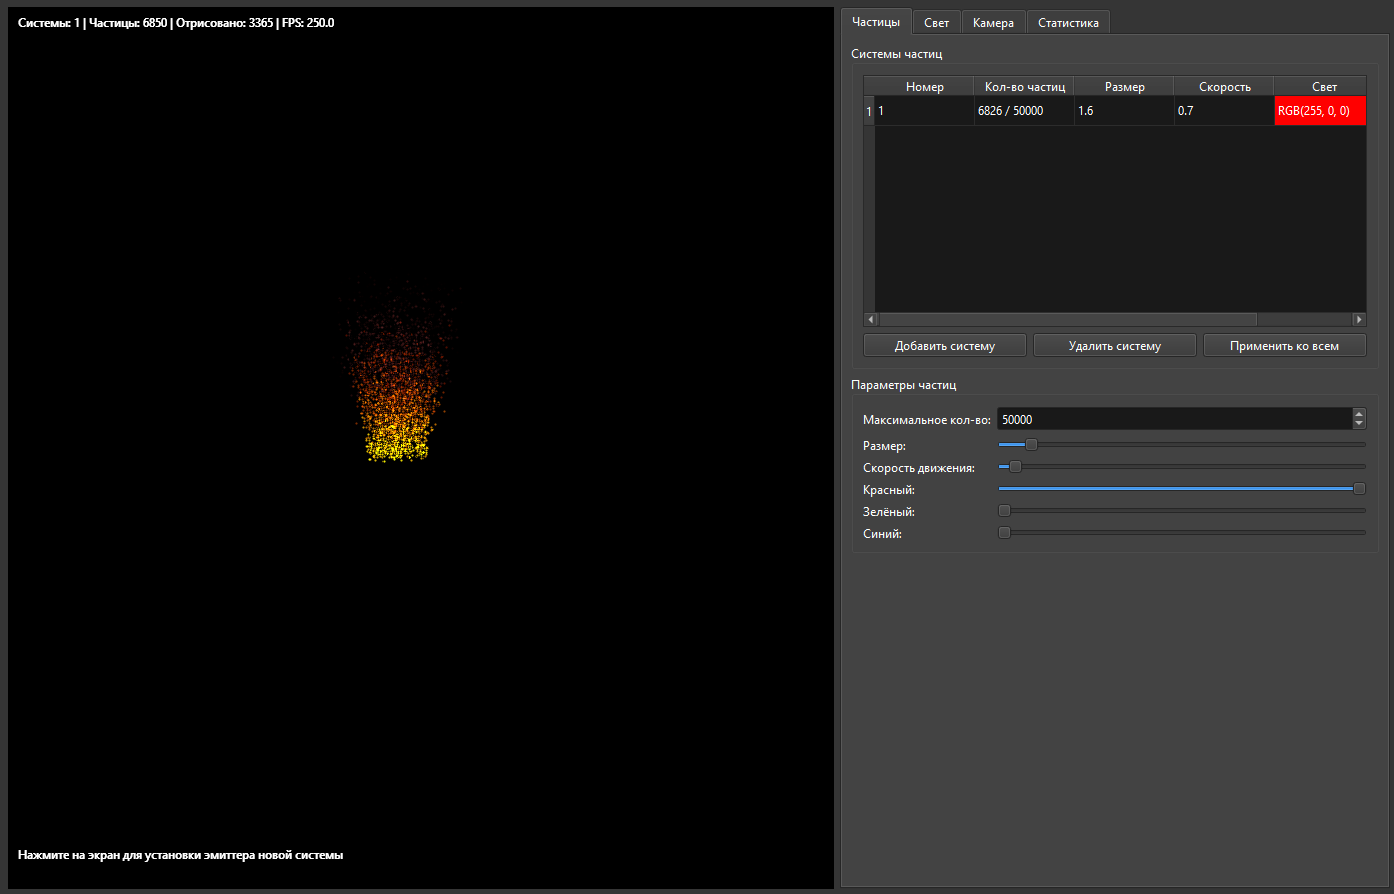
\includegraphics[width=0.7\textwidth]{research_1.png}
	\caption{Визуализация одной системы частиц}
	\label{fig:research-1}
\end{figure}

\begin{figure}[h!]
	\centering
	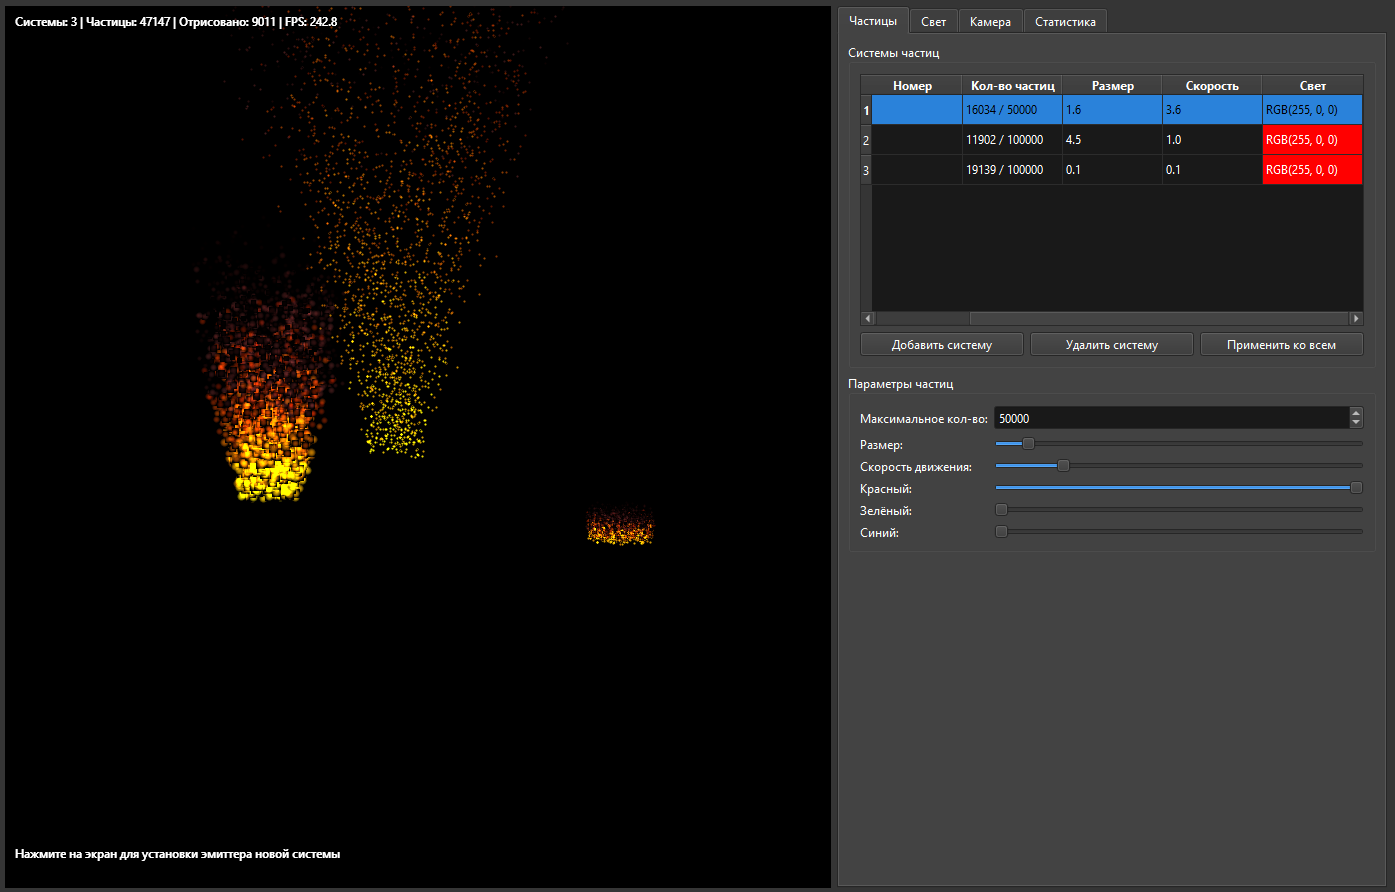
\includegraphics[width=0.7\textwidth]{research_2.png}
	\caption{Несколько систем частиц с разными параметрами}
	\label{fig:research-2}
\end{figure}

\clearpage

\begin{figure}[h!]
	\centering
	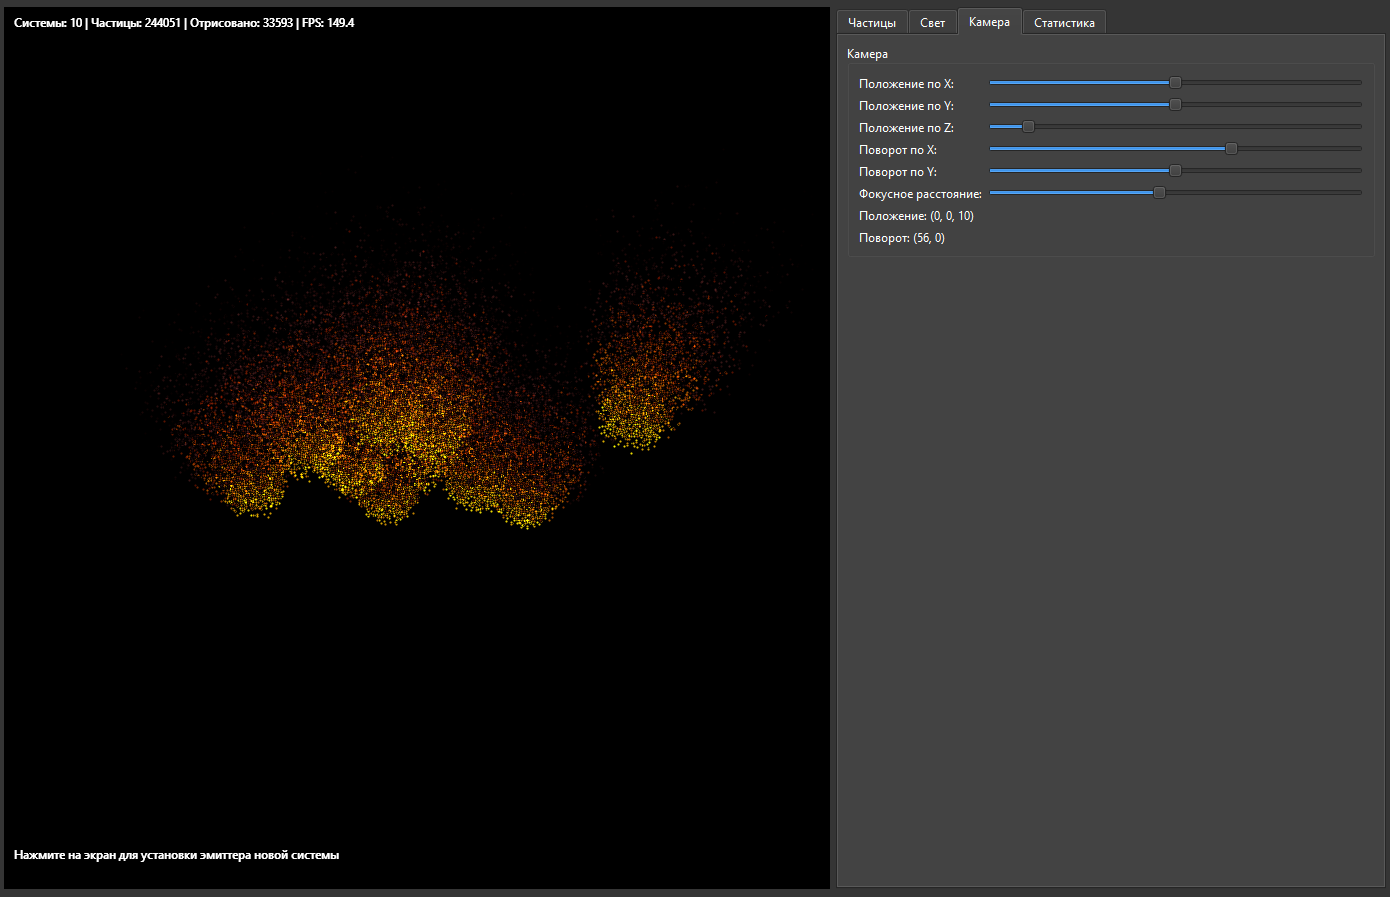
\includegraphics[width=0.7\textwidth]{research_3.png}
	\caption{Изменение ракурса камеры}
	\label{fig:research-3}
\end{figure}

\begin{figure}[h!]
	\centering
	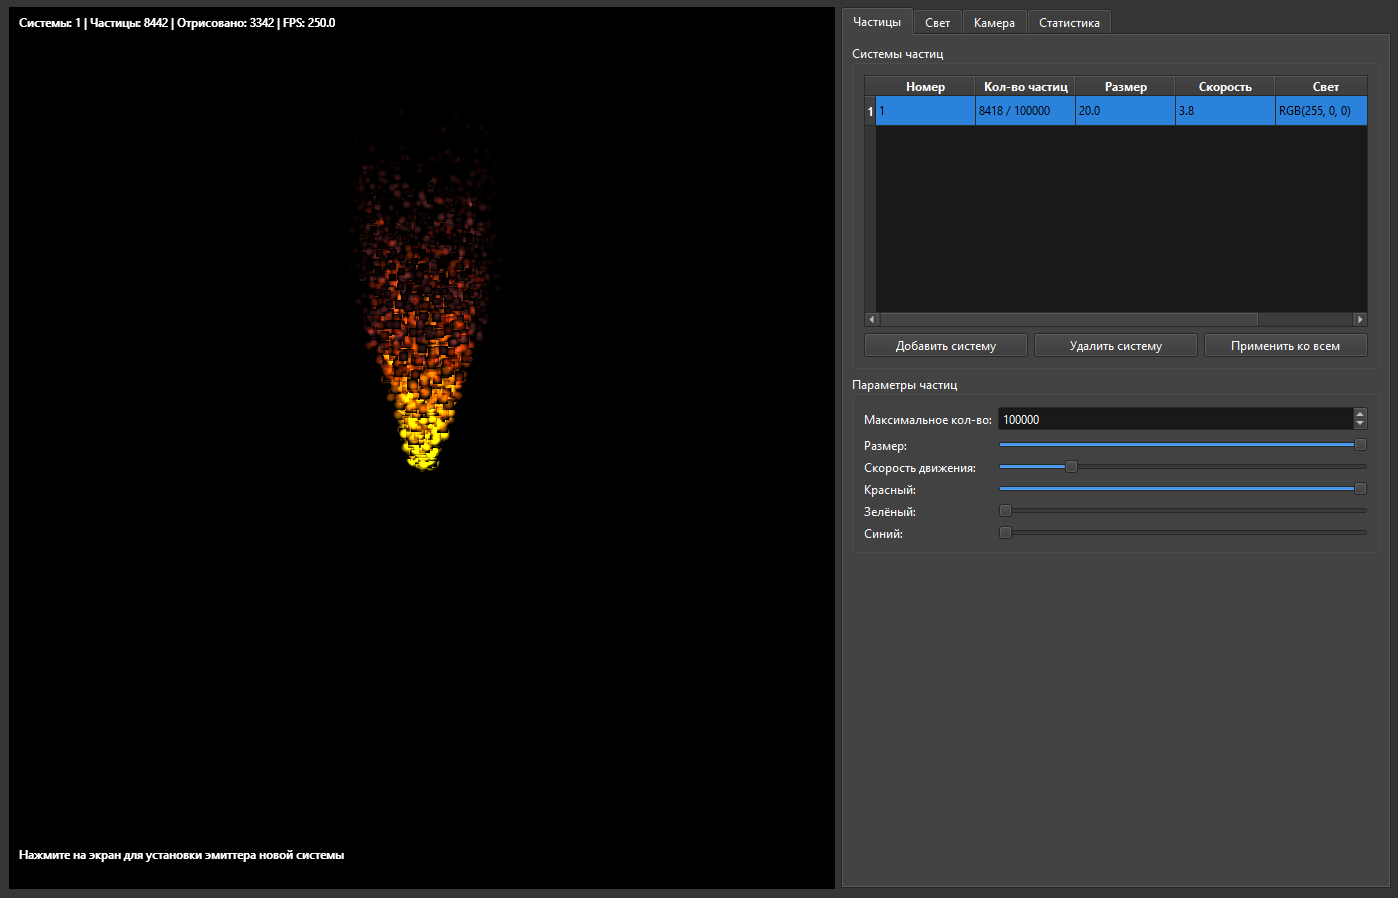
\includegraphics[width=0.7\textwidth]{research_4.png}
	\caption{Увеличенный размер частиц}
	\label{fig:research-4}
\end{figure}

\clearpage

\begin{figure}[h!]
	\centering
	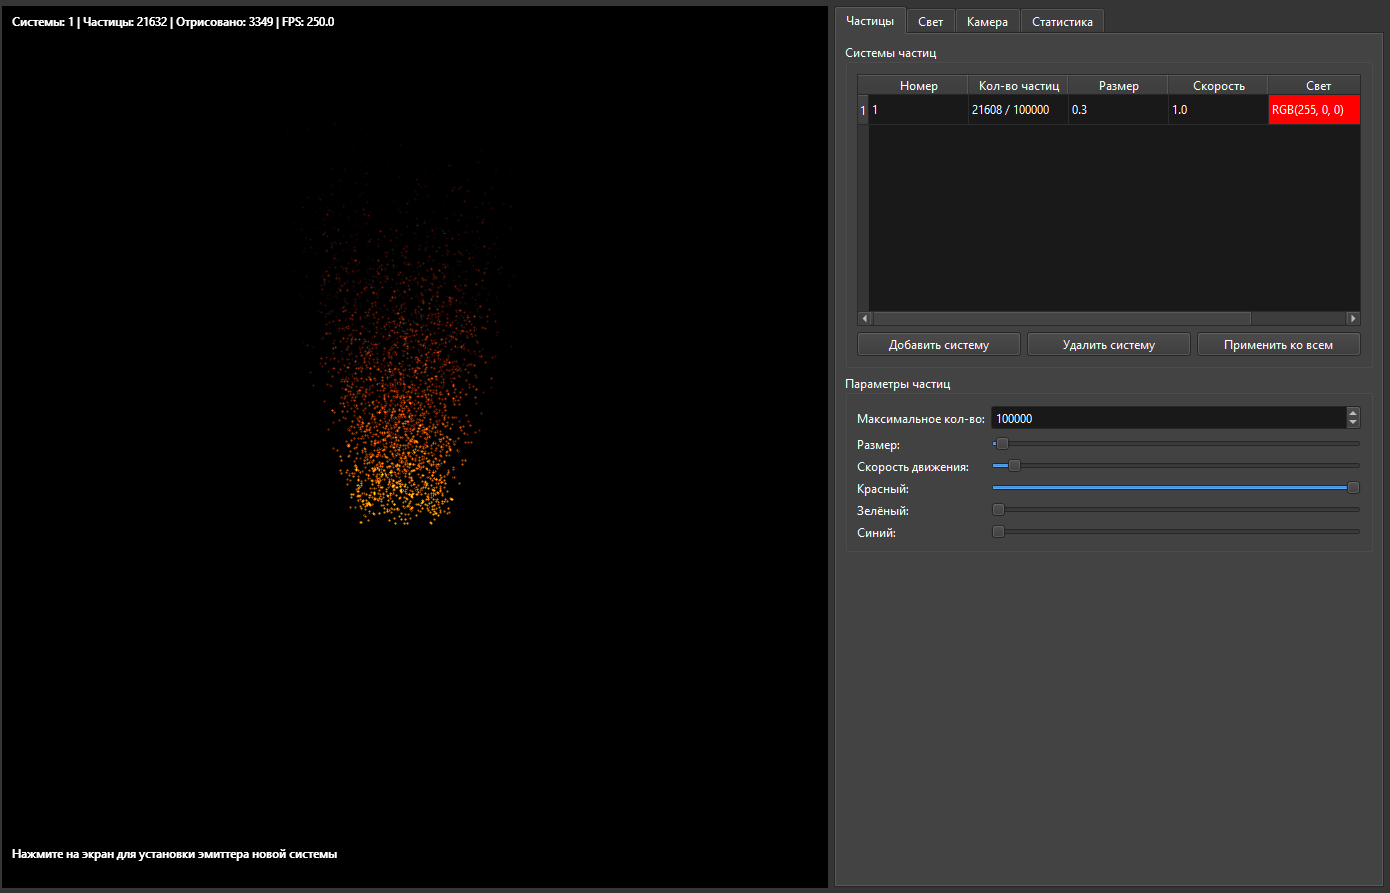
\includegraphics[width=0.7\textwidth]{research_5.png}
	\caption{Визуализация без внешнего освещения}
	\label{fig:research-5}
\end{figure}

\begin{figure}[h!]
	\centering
	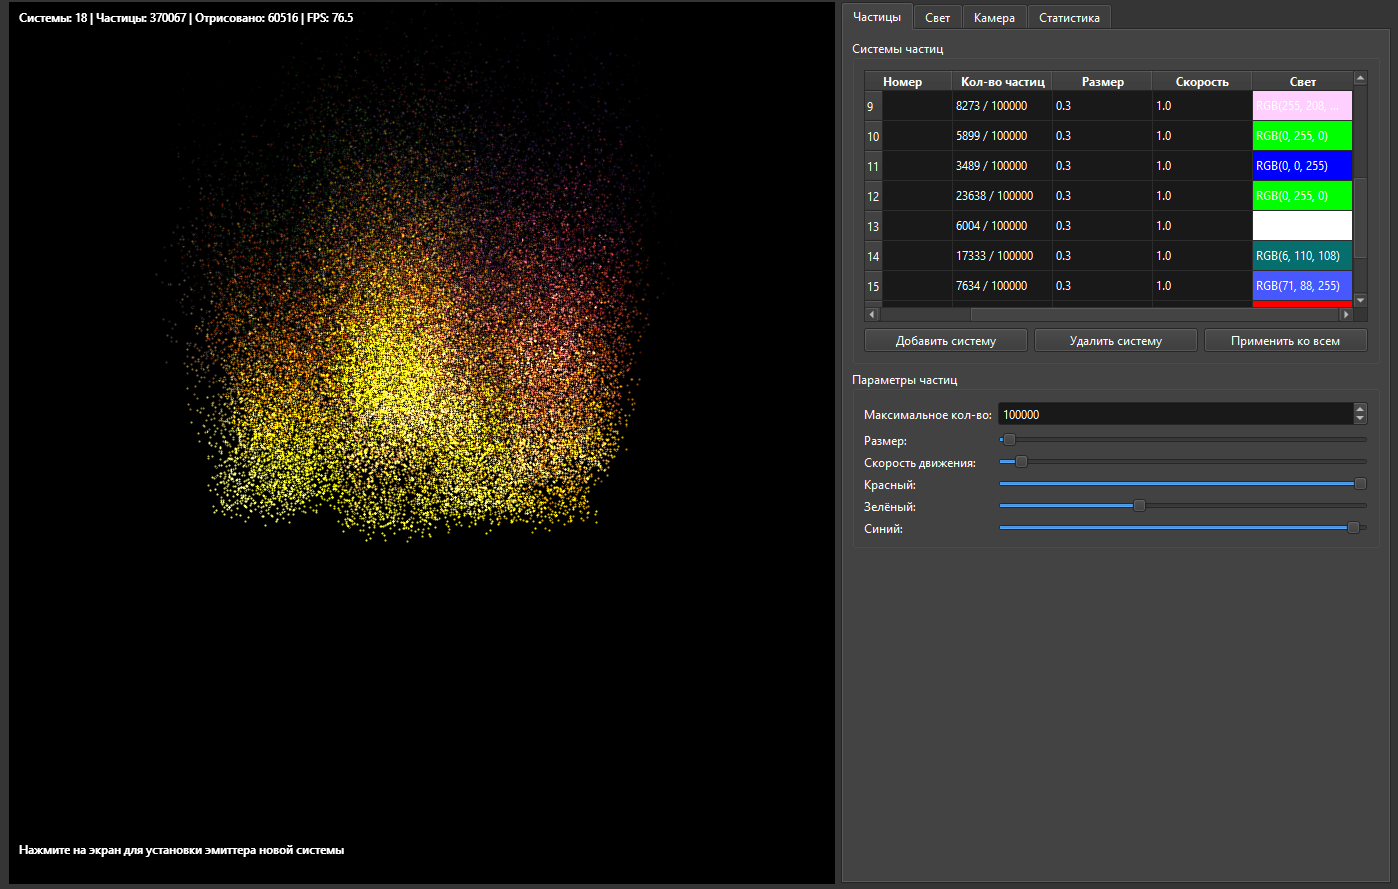
\includegraphics[width=0.7\textwidth]{research_6.png}
	\caption{Визуализация множества систем различного цвета}
	\label{fig:research-6}
\end{figure}

\section{Вывод}
В технологической части разработана архитектура программного комплекса для визуализации трёхмерного огня. Выбран язык программирования C++ и фреймворк Qt для реализации. Разработана объектно-ориентированная архитектура с разделением ответственности между классами. Реализованы ключевые алгоритмы.

Создан графический интерфейс с разделением на логические блоки управления. Обеспечена возможность интерактивного управления сценой в реальном времени со статистикой производительности.
\clearpage